\documentclass[conference]{IEEEtran}
\IEEEoverridecommandlockouts
% The preceding line is only needed to identify funding in the first footnote. If that is unneeded, please comment it out.
\usepackage{cite}
\usepackage{amsmath,amssymb,amsfonts}
\usepackage{algorithmic}
\usepackage{graphicx}
\usepackage{textcomp}
\usepackage{xcolor}
\def\BibTeX{{\rm B\kern-.05em{\sc i\kern-.025em b}\kern-.08em
    T\kern-.1667em\lower.7ex\hbox{E}\kern-.125emX}}
\begin{document}

\title{Szakdolgozati beszámoló\\

\thanks{}
}

\author{\IEEEauthorblockN{Pekár Mihály}
\IEEEauthorblockA{\textit{PTI bsc.} \\
\textit{Eszterházy Károly Egyetem}\\
Eger, Magyarország \\
mpekar55@gmail.com}
}

\maketitle

\begin{abstract}
Ebben a dokumentumban arról fogok írni, hogy a jelenlegi félévben milyen feladatokat tudtam teljesíteni a szakdolgozatom megírásában illetve, hogy nehézségekbe ütköztem ezalatt. Továbbá azt is befogom még mutatni, hogy mik várnak még rám a szakdolgozatom befejeztéig. 
\end{abstract}

\begin{IEEEkeywords}
iktatás, szakdolgozat, grpc, mysql, protobuf
\end{IEEEkeywords}

\section{Bevezetés}
Ez egy bevezetés lesz ahol is kontextusba kell helyeznem a dokumentumot ami foglamam sincs, hogy mit jelent, de remélem hamarosan okosabb leszek. :)

\section{Féléves munka bemutatása}

\subsection{\textbf{Igényfelmérés}}

The IEEEtran class file is used to format your paper and style the text. All margins, 
column widths, line spaces, and text fonts are prescribed; please do not 
alter them. You may note peculiarities. For example, the head margin
measures proportionately more than is customary. This measurement 
and others are deliberate, using specifications that anticipate your paper 
as one part of the entire proceedings, and not as an independent document. 
Please do not revise any of the current designations.


\subsection{\textbf{Adatbázis tervezése és megvalósítása}}


\subsubsection{\textbf{Táblák}}
\begin{figure}[htbp]
	\centerline {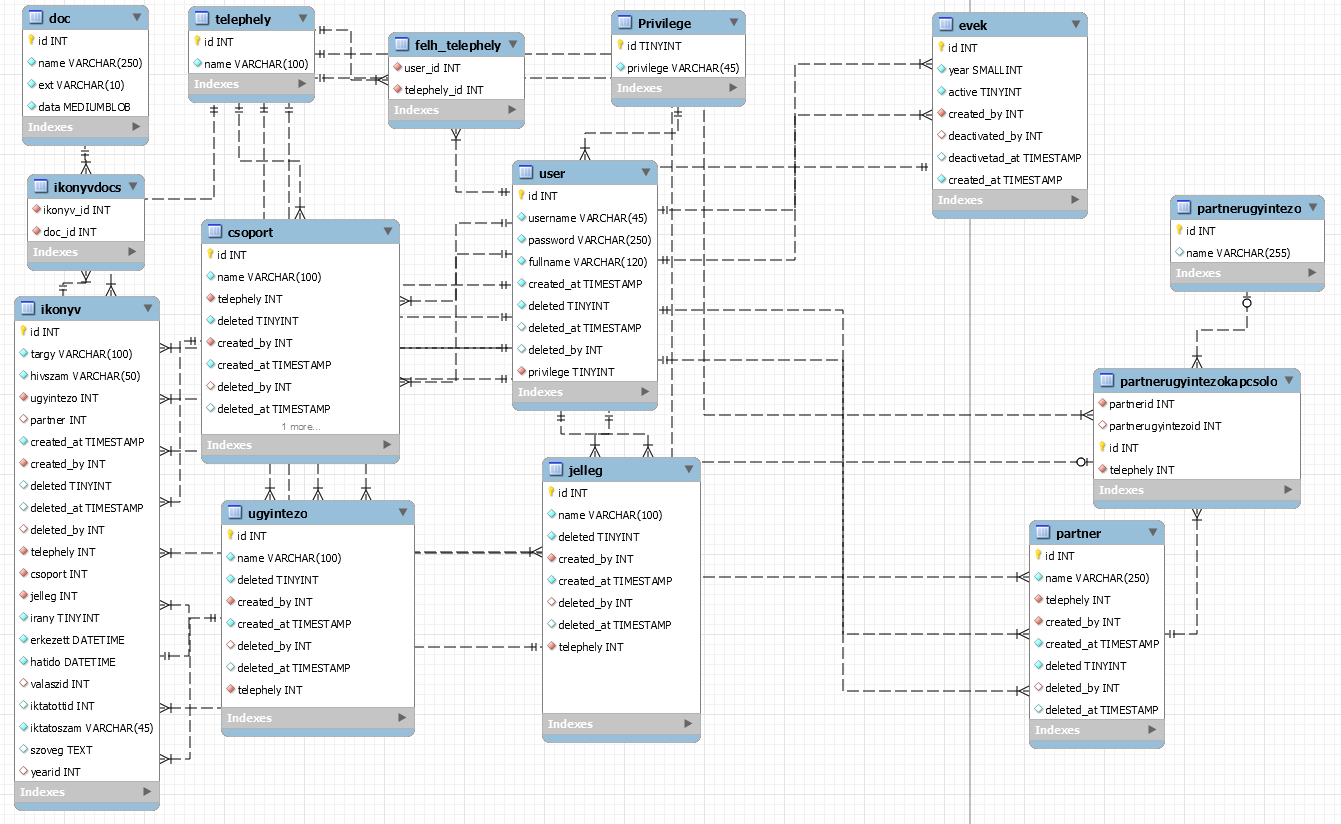
\includegraphics[width=8cm,height=8cm,keepaspectratio]{adatbazis.png}}
	\caption{Adatbázis képe mysql workbenchben programban}
	\label{fig1}
\end{figure}
\begin{itemize}
	\item Évek:
	Az aktív évet jeleníti meg a programban, hogy melyik évre iktatunk. Év zárása után már nem lehet arra az évre iktatni.
	\item User tábla:
	A programot használó dolgozók adatait tartalmazza. Három oszlopból áll. Felhasználónév aminek a maximális mérete 45 karakterhosszú. Jelszó ami SHA1 kódolással lesz eltárolva, illetve a felhasználó teljese neve.
	\item Privilege:
	A felhasználó jogosultásgi szintje a programban. Lehet Admin és User. Az admin jogosultsággal rendelkezők a törzseket szabadon szerkeszthetik, felhasználókat adhatnak , módosíthatnak vagy törölhetnek a rendszerben illetve "törölhetnek" iktatásokat.
	Míg a sima felhasználó iktatáson kívül még partnert, partner ügyintézőt és ügyintézőket tud csak hozzáadni a rendszerhez.
	\item Telephely:
	Ez jelöli, hogy az adat az melyik telephelyhez tartozik az adatbázisban. Ez vonatkozik az iktatásra és a törzsadatokra egyaránt.	
	\item Felhtelephely:	
	Minden felhasználóhoz tartozik egy vagy több telephely ahová tud iktatni vagy törzs adatokat rögzíteni. 
	\item Partner:	
	Azokat a partnereket tartalmazza akiket a
	\item Partnerügyintéző:
	A megadott partnerhez tartozó ügyintézőket tartalmazza
	\item Partnerügyintéző kapcsoló:
	Az a személy, intézmény vagy cég aki küldte az iratot. Munkaszerződéseknél a partner a dolgozó nevét jelöli. Lehet például E-on, Járási hivatal..stb. Ennek a táblának az id-je fog idegen kulcsként megjelenni az iktatásban.
	\item Csoport
	Az iratok azon típusait jelöli, amely egységhez kapcsolódik az iktatandó anyag. Például Ellátotti, Főzőkonyha, Munkaügy.
	\item Jelleg
	A dokumentum formai megjelenésének megadása. Ez lehet e-mail, küldemény, fax, levél, munkaügyi irat.
	\item Ügyintéző	
	Ez a szervezeten belüli dolgozó kollégára utal, hogy ezt az ügyet vagy iratot ki intézi.
	\item Doc
	Itt tároljuk az iktatásokhoz feltöltött állományokat mediumblobban. Illetve eltároljuk még annak nevét és a kiterjesztését is. Lehet Pdf,JPG,PNG,XLSX,DOCX...stb.
	\item Ikonyv docs
	Az adott iktatáshoz tartozó dokumentum.
	\item Ikonyv
	Ez maga az iktató könyv. Ha bejön egy irat vagy kimegy azt itt lesz rögzítve. Az iktatószámot tárolt eljárással fogom előállítani ami a megadott adatok alapján fog generálódni. Egy példa: B-SZ/R/3/2019 Ennek felépítése
	\begin{itemize}
		\item Az első karakteret az határozza meg, hogy K - kimenő vagy B - bejövő
		\item A második karakter a jellege határozza meg SZ pl szerződés.
		\item A harmadik karakter a telephely jelöli pl. R - Rákóczi, V- Vajda stb..
		\item A negyedik karakter sorozat a sorszám ami lehet kötőjeles Pl. B-SZ/R/3-1/2019 vagy B-SZ/R/3-1-1/2019 a válaszokhoz mérve.
		\item Az utolsó rész pedig az évet jelöli.
		
	\end{itemize}
	Az iktatószám generálása után el is lesz tárolva.
	
\end{itemize}
\subsubsection{\textbf{Views}}
Number equations consecutively. To make your 
equations more compact, you may use the solidus (~/~), the exp function, or 
appropriate exponents. Italicize Roman symbols for quantities and variables, 
but not Greek symbols. Use a long dash rather than a hyphen for a minus 
sign. Punctuate equations with commas or periods when they are part of a 
sentence, as in:
\begin{equation}
a+b=\gamma\label{eq}
\end{equation}

Be sure that the 
symbols in your equation have been defined before or immediately following 
the equation. Use ``\eqref{eq}'', not ``Eq.~\eqref{eq}'' or ``equation \eqref{eq}'', except at 
the beginning of a sentence: ``Equation \eqref{eq} is . . .''

\subsubsection{\textbf{Tárolt eljárások}}

Minden kérést amit lehetett tárolt eljárásba tettem. Ezzel is megakadályozva az SQL injectionnek a lehetőségét. Összesen 39 darab lett belőlük, de ezeknek a száma valószínűleg csak növekedni fog az iktató program fejlesztése során mivel előfordulhatnak olyan lekérdezések amikre még nem gondoltam a tervezés során.
Pár fontosabb eljárást fogok csak bemutatni, mivel a nagy része csak az adatok megfelelő módosításáról, törléséről és hozzáadásáról szól. A legfontosabbak a következők.
AddRootIkonyv, AddSubIkonyv, DelIkonyv, setDeletedByValaszID, getNextIktatottID, getIkonyvek. Ezek okozták a legtöbb fejtörést a számomra.
 
\begin{itemize}
	\item AddRootIkonyv:
	\item AddSubIkonyv:
	\item DelIkonyv:
	\item setDeletedByValaszID:
	\item getNextIktatottID:
	\item getIkonyvek:
\end{itemize} 

Az adatbázisnak a megtervezésekor mindent információt figyelembe vettem amit az igényfelmérés során összegyűjtöttem. Reményeim szerint nem fog kelleni sok mindent újra tervezni mikor csinálom a gRPC szervert illetve a felhasználó felületet. Amit már biztosan tudok, hogy az adatbázisban még van egy probléma méghozzá a partnereknek a tárolása amit még újra kell gondolnom.
\subsection{\textbf{gRPC és Protocol Buffers}}
\textbf{Grpc:}
GRPC-ről egy rövid leírás és hogy meddig jutottam vele.

\textbf{Protocol Buffer:}
\subsubsection{Osztályok}

\subsubsection{Metódusok}


\subsubsection{Függvények}



\section*{Feladatok, tervek és azok kivitelezése a szakdolgozat befejezéséig.}



\section*{Eredmények}


\begin{thebibliography}{00}
\bibitem{b1} G. Eason, B. Noble, and I. N. Sneddon, ``On certain integrals of Lipschitz-Hankel type involving products of Bessel functions,'' Phil. Trans. Roy. Soc. London, vol. A247, pp. 529--551, April 1955.
\bibitem{b2} J. Clerk Maxwell, A Treatise on Electricity and Magnetism, 3rd ed., vol. 2. Oxford: Clarendon, 1892, pp.68--73.
\bibitem{b3} I. S. Jacobs and C. P. Bean, ``Fine particles, thin films and exchange anisotropy,'' in Magnetism, vol. III, G. T. Rado and H. Suhl, Eds. New York: Academic, 1963, pp. 271--350.
\bibitem{b4} K. Elissa, ``Title of paper if known,'' unpublished.
\bibitem{b5} R. Nicole, ``Title of paper with only first word capitalized,'' J. Name Stand. Abbrev., in press.
\bibitem{b6} Y. Yorozu, M. Hirano, K. Oka, and Y. Tagawa, ``Electron spectroscopy studies on magneto-optical media and plastic substrate interface,'' IEEE Transl. J. Magn. Japan, vol. 2, pp. 740--741, August 1987 [Digests 9th Annual Conf. Magnetics Japan, p. 301, 1982].
\bibitem{b7} M. Young, The Technical Writer's Handbook. Mill Valley, CA: University Science, 1989.
\end{thebibliography}
\vspace{12pt}

\end{document}
